\documentclass[tikz,border=10pt]{standalone}
% Shared look for every TikZ diagram. Load with % Shared look for every TikZ diagram. Load with % Shared look for every TikZ diagram. Load with \input{../../tools/tikz-style.tex}
\usepackage[T1]{fontenc}
\usepackage{lmodern}
\renewcommand{\sfdefault}{lmr}  % diagrams use the same serif as the text
\usetikzlibrary{arrows.meta, positioning, shapes.geometric, calc, fit, backgrounds}
\definecolor{cblue}{HTML}{4C78A8}
\definecolor{corange}{HTML}{F58518}
\definecolor{cgreen}{HTML}{54A24B}
\definecolor{cred}{HTML}{E45756}
\definecolor{cpurple}{HTML}{B279A2}
\definecolor{cgrey}{HTML}{6B6B6B}
\tikzset{
  every picture/.style={font=\sffamily, line width=1.2pt},
  box/.style={draw=#1, fill=#1!12, rounded corners=4pt, align=center, inner sep=7pt, minimum height=1.1cm},
  box/.default=cgrey,
  arrow/.style={-{Stealth[length=3mm]}, draw=cgrey, line width=1.4pt},
  title/.style={font=\sffamily\bfseries\Large},
  note/.style={font=\sffamily\small, text=cgrey, align=center},
}
\AtBeginDocument{\hyphenpenalty=10000 \exhyphenpenalty=10000}

\usepackage[T1]{fontenc}
\usepackage{lmodern}
\renewcommand{\sfdefault}{lmr}  % diagrams use the same serif as the text
\usetikzlibrary{arrows.meta, positioning, shapes.geometric, calc, fit, backgrounds}
\definecolor{cblue}{HTML}{4C78A8}
\definecolor{corange}{HTML}{F58518}
\definecolor{cgreen}{HTML}{54A24B}
\definecolor{cred}{HTML}{E45756}
\definecolor{cpurple}{HTML}{B279A2}
\definecolor{cgrey}{HTML}{6B6B6B}
\tikzset{
  every picture/.style={font=\sffamily, line width=1.2pt},
  box/.style={draw=#1, fill=#1!12, rounded corners=4pt, align=center, inner sep=7pt, minimum height=1.1cm},
  box/.default=cgrey,
  arrow/.style={-{Stealth[length=3mm]}, draw=cgrey, line width=1.4pt},
  title/.style={font=\sffamily\bfseries\Large},
  note/.style={font=\sffamily\small, text=cgrey, align=center},
}
\AtBeginDocument{\hyphenpenalty=10000 \exhyphenpenalty=10000}

\usepackage[T1]{fontenc}
\usepackage{lmodern}
\renewcommand{\sfdefault}{lmr}  % diagrams use the same serif as the text
\usetikzlibrary{arrows.meta, positioning, shapes.geometric, calc, fit, backgrounds}
\definecolor{cblue}{HTML}{4C78A8}
\definecolor{corange}{HTML}{F58518}
\definecolor{cgreen}{HTML}{54A24B}
\definecolor{cred}{HTML}{E45756}
\definecolor{cpurple}{HTML}{B279A2}
\definecolor{cgrey}{HTML}{6B6B6B}
\tikzset{
  every picture/.style={font=\sffamily, line width=1.2pt},
  box/.style={draw=#1, fill=#1!12, rounded corners=4pt, align=center, inner sep=7pt, minimum height=1.1cm},
  box/.default=cgrey,
  arrow/.style={-{Stealth[length=3mm]}, draw=cgrey, line width=1.4pt},
  title/.style={font=\sffamily\bfseries\Large},
  note/.style={font=\sffamily\small, text=cgrey, align=center},
}
\AtBeginDocument{\hyphenpenalty=10000 \exhyphenpenalty=10000}

\begin{document}
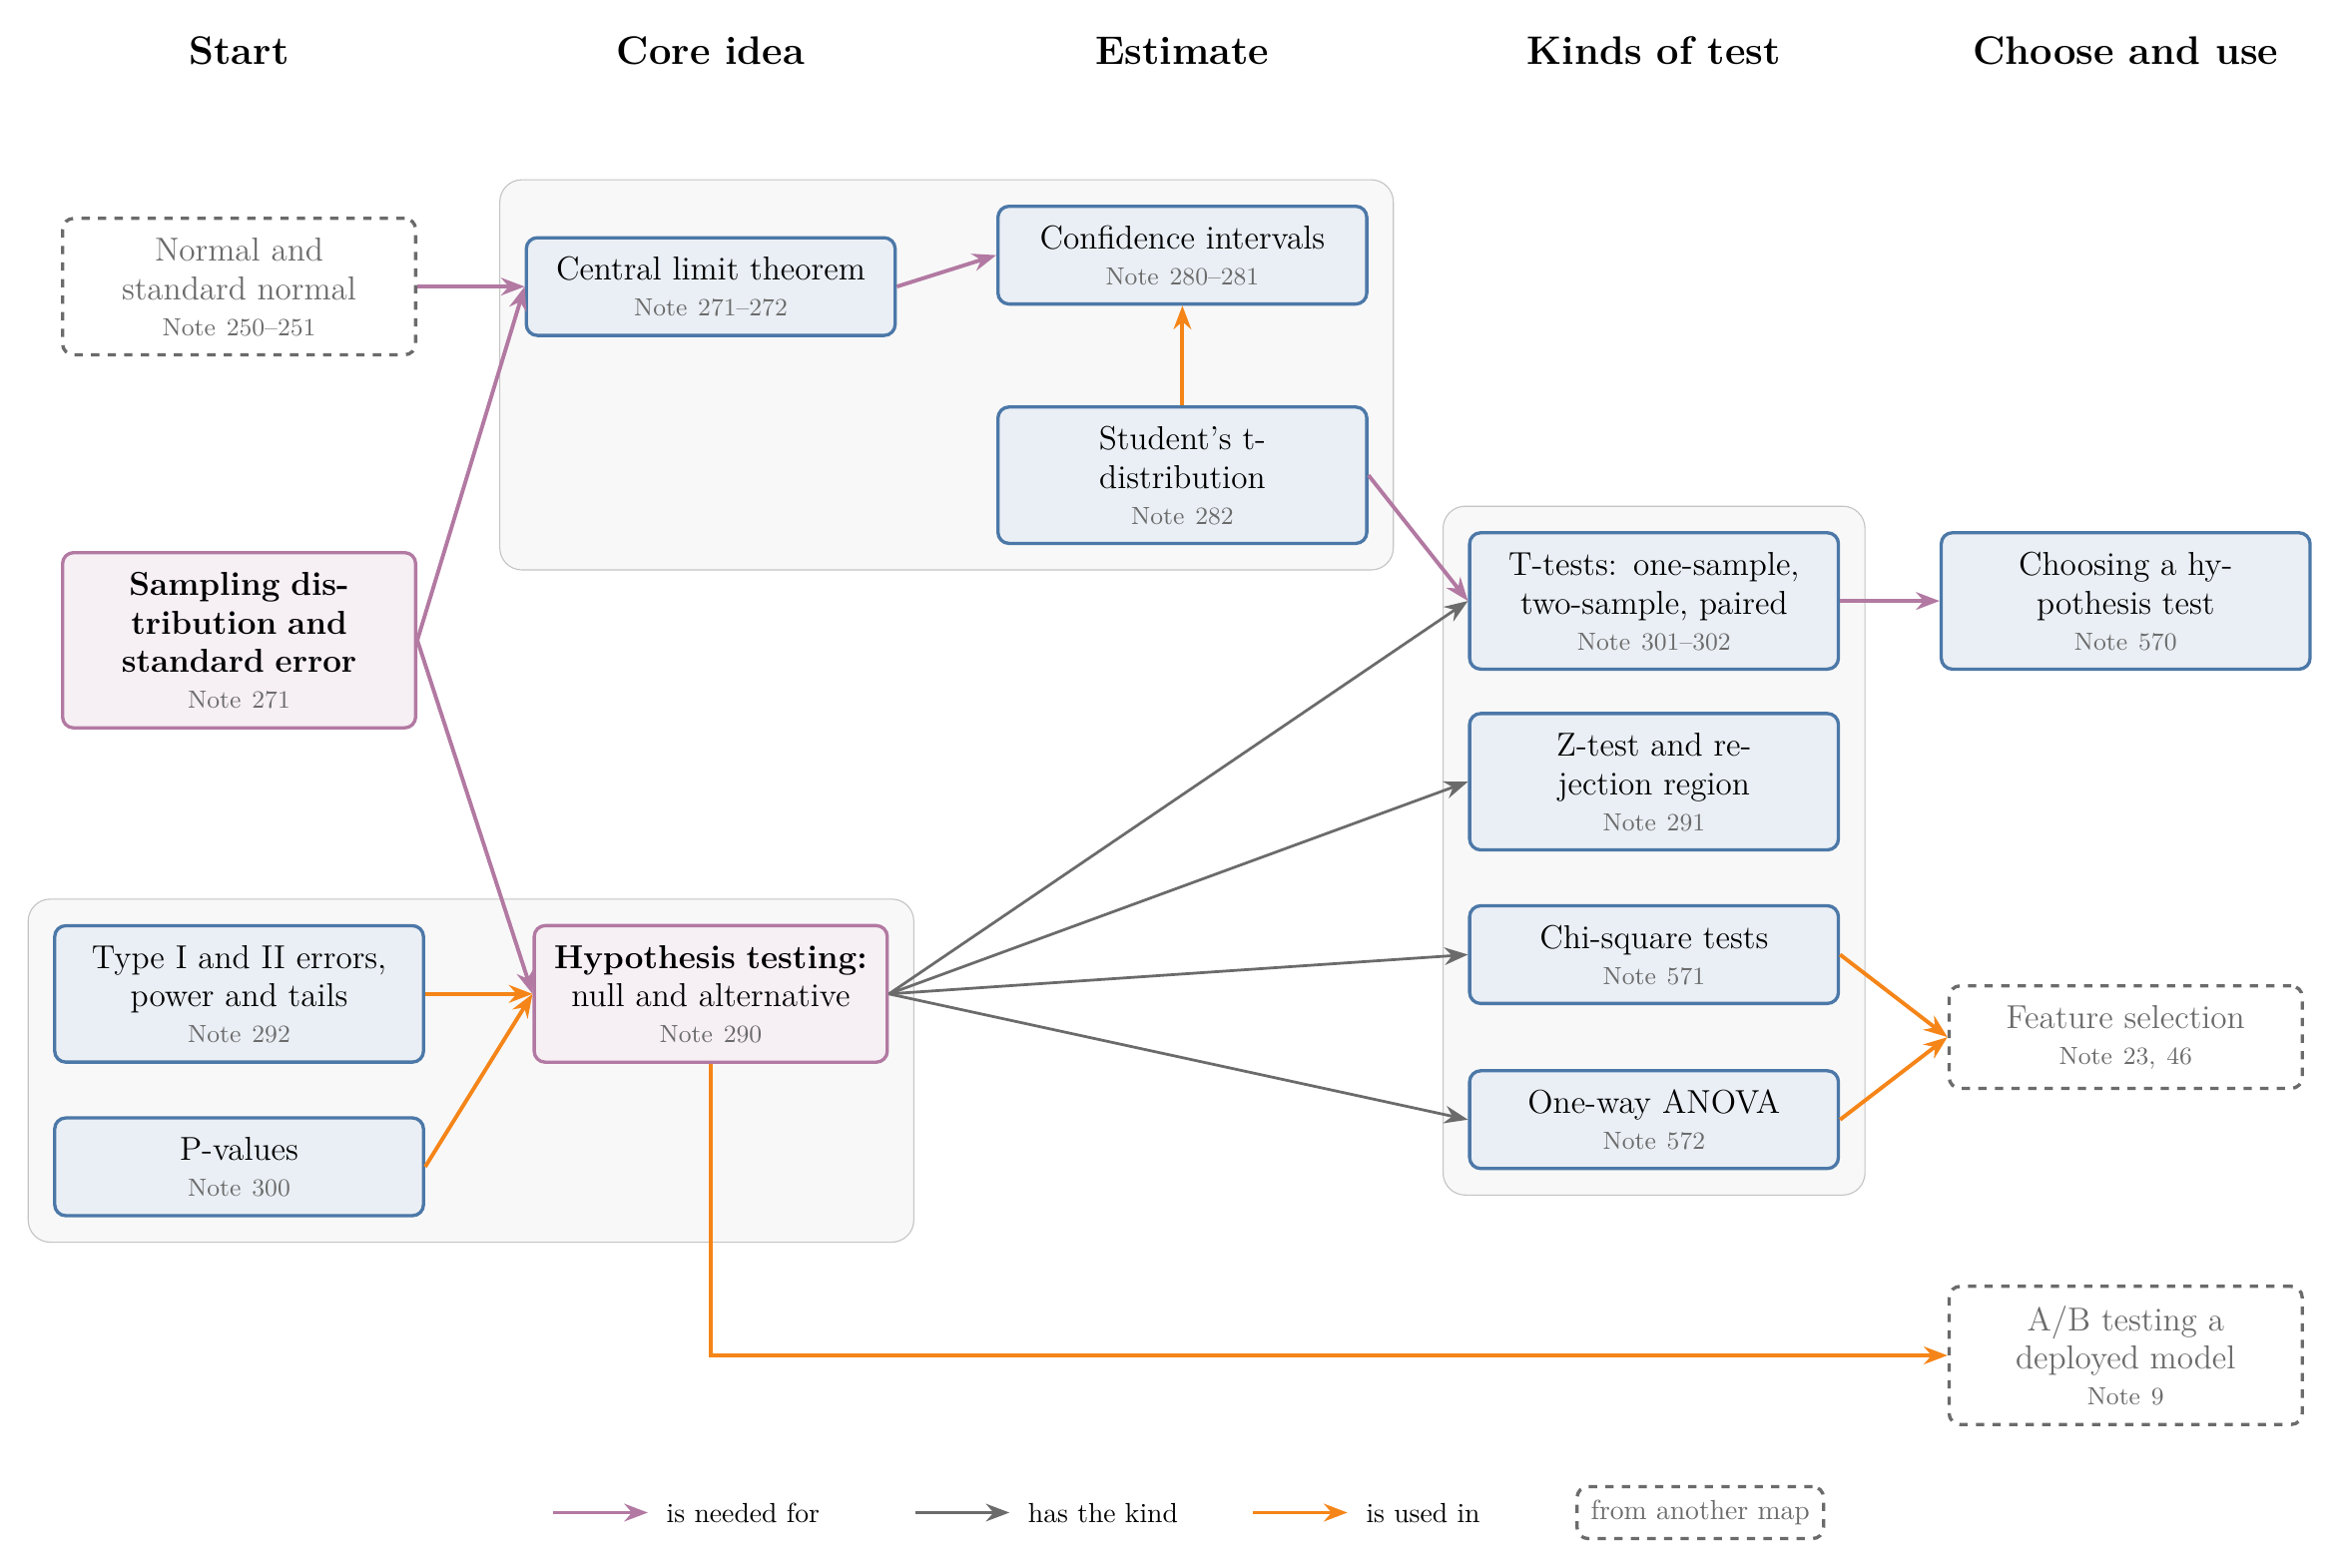
\begin{tikzpicture}[
    every node/.append style={font=\sffamily\large},
    idea/.style={box=cpurple, text width=4.0cm},
    con/.style={box=cblue, text width=4.2cm},
    prev/.style={draw=cgrey, dashed, rounded corners=4pt, align=center, inner sep=7pt, text=cgrey, text width=4.0cm, minimum height=1.1cm},
    group/.style={draw=cgrey!40, fill=cgrey!5, rounded corners=8pt, inner sep=9pt},
    needs/.style={arrow, draw=cpurple},
    kind/.style={arrow, draw=cgrey, line width=1pt},
    used/.style={arrow, draw=corange},
  ]
  \newcommand{\nt}[1]{\\[-1pt]{\small\color{cgrey}Note #1}}
  \node[title] at (0,9.0)  {Start};
  \node[title] at (6,9.0)  {Core idea};
  \node[title] at (12,9.0) {Estimate};
  \node[title] at (18,9.0) {Kinds of test};
  \node[title] at (24,9.0) {Choose and use};

  % start
  \node[prev] (nor)  at (0,6.0)  {Normal and standard normal\nt{250--251}};
  \node[idea] (samp) at (0,1.5)  {\textbf{Sampling distribution and standard error}\nt{271}};
  \node[con]  (err)  at (0,-3.0) {Type I and II errors, power and tails\nt{292}};
  \node[con]  (pval) at (0,-5.2) {P-values\nt{300}};

  % core ideas
  \node[con]  (clt)  at (6,6.0)  {Central limit theorem\nt{271--272}};
  \node[idea] (ht)   at (6,-3.0) {\textbf{Hypothesis testing:} null and alternative\nt{290}};

  % estimate
  \node[con]  (ci)   at (12,6.4) {Confidence intervals\nt{280--281}};
  \node[con]  (td)   at (12,3.6) {Student's t-distribution\nt{282}};

  % kinds of test
  \node[con]  (tt)   at (18,2.0)  {T-tests: one-sample, two-sample, paired\nt{301--302}};
  \node[con]  (zt)   at (18,-0.3) {Z-test and rejection region\nt{291}};
  \node[con]  (chi)  at (18,-2.5) {Chi-square tests\nt{571}};
  \node[con]  (an)   at (18,-4.6) {One-way ANOVA\nt{572}};

  % choose and use
  \node[con]  (ch)   at (24,2.0)  {Choosing a hypothesis test\nt{570}};
  \node[prev] (fs)   at (24,-3.55) {Feature selection\nt{23, 46}};
  \node[prev] (ab)   at (24,-7.6)  {A/B testing a deployed model\nt{9}};

  \begin{scope}[on background layer]
    \node[group, fit=(clt) (ci) (td)] {};
    \node[group, fit=(err) (pval) (ht)] {};
    \node[group, fit=(tt) (an)] {};
  \end{scope}

  % estimation
  \draw[needs] (nor.east) -- (clt.west);
  \draw[needs] (samp.east) -- (clt.west);
  \draw[needs] (clt.east) -- (ci.west);
  \draw[used]  (td.north) -- (ci.south);

  % testing
  \draw[needs] (samp.east) -- (ht.west);
  \draw[used]  (err.east) -- (ht.west);
  \draw[used]  (pval.east) -- (ht.west);
  \foreach \k in {tt, zt, chi, an} \draw[kind] (ht.east) -- (\k.west);
  \draw[needs] (td.east) -- (tt.west);
  \draw[needs] (tt.east) -- (ch.west);
  \draw[used]  (chi.east) -- (fs.west);
  \draw[used]  (an.east) -- (fs.west);
  \draw[used]  (ht.south) |- (ab.west);

  % legend
  \begin{scope}[shift={(4.0,-9.6)}, every node/.style={font=\sffamily, anchor=west}]
    \draw[needs] (0,0) -- (1.2,0);     \node at (1.3,0) {is needed for};
    \draw[kind] (4.6,0) -- (5.8,0);    \node at (5.9,0) {has the kind};
    \draw[used] (8.9,0) -- (10.1,0);   \node at (10.2,0) {is used in};
    \node[draw=cgrey, dashed, rounded corners=4pt, inner sep=5pt, text=cgrey, anchor=west] at (13.0,0) {from another map};
  \end{scope}
\end{tikzpicture}
\end{document}
